\begin{frame}{Fitnessberechnung}
    \begin{columns}[T] % T aligns the tops of the columns
        \begin{column}{0.55\textwidth}
            \vspace*{0.2cm}
            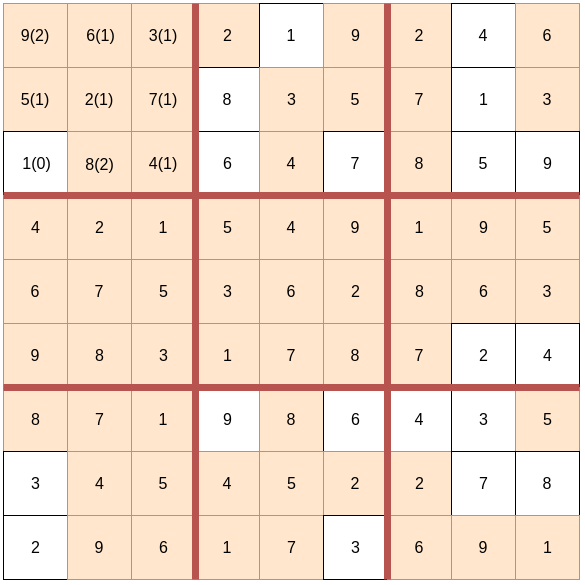
\includegraphics[width=\textwidth]{Pictures/Collision-Fitness.png}
        \end{column}
        \begin{column}{0.55\textwidth}
            \begin{itemize}
                \vspace*{0.25cm}
                \item Berechnen der individuellen Kollisionen
                \item Anlegen eines "{}Fitness-Sudokus{}" zur Speicherung der Werte \\
                \(\rightarrow\) Mutation (s. Block 0) 
                \item Kollisionszahl als Fitnesswert (=86)
                \item 0 als Idealwert entspricht gelöstem Sudoku
            \end{itemize}
        \end{column}
    \end{columns}
\end{frame}
